% synthesis

% Overview paragraph
%     summarizing importance of S.L.R.
%     why does the RIS matter?
%     what are the geologic controls on RIS stability?

Improving decadal to centennial projections of global sea level rise is of utmost importance for mitigating future environment and socio-economic impacts \citep{durandsealevel2022}. 
Antarctica's projected contributions to global sea level rise by the end of the century under a high-emission scenario is between 0.03 and 0.28~m \citep[RCP 8.5,][]{intergovernmentalpanelonclimatechangeipccocean2022}. 
This wide range of possible values expresses the uncertainty of the Antarctic Ice Sheet's response to a warming world. 
Over 80\% of ice loss from Antarctica occurs through ice shelves \citep{rignoticeshelf2013}, highlighting their importance in reducing the uncertainty in sea level rise projections. 
Antarctica's largest ice shelf, the Ross Ice Shelf, is fed from both the East and West Antarctic Ice Sheets. 
Its catchment contains a total volume of ice equivalent to 11.6~m of global sea level rise \citep{fretwellbedmap22013, rignotantarctic2011, tintoross2019}. 
While the Ross Ice Shelf is relatively stable currently \citep{moholdtbasal2014, rignoticeshelf2013}, geologic evidence shows the rapid destabilization of the ice shelf within the past $\sim$7,000 years \citep[e.g.,][]{venturellimid2020, naishobliquitypaced2009}. \\

The destabilization of the ice shelf is thought to have been primarily caused by ocean forcings \citep{lowrydeglacial2019}, as bathymetric troughs guide the inflow of melt-inducing ocean circulations \citep{tintoross2019}. 
The subsequent grounding line retreat however is predominantly controlled by the physiography, geology, and glaciological feedbacks \citep{halberstadticesheet2016}. 
This highlights the solid earth, through its bathymetric control on basal melt and its effects on grounding line retreat dynamics, as an important component of the dynamics of the Ross Ice Shelf. 
To reliably understand the contribution of the Ross Ice Shelf to future sea level rise, we must provide ocean and ice modellers with the necessary geologic boundary conditions. 
This thesis aimed to provide both these boundary conditions and estimates of their uncertainties to the modelling community. 
A series of research questions were proposed, as restated below.

\begin{enumerate}
    \item 
        What is the geologic structure of the upper crust beneath the Ross Ice Shelf? 
        If there are sediments, what is their thickness and distribution? 
        Where are the major faults likely located? 
    \item 
        How can bathymetry beneath an ice shelf best be modelled? 
        Are there further improvements that can be made to the gravity-inversion process? 
        What are the predominant sources of uncertainty, and how can these be limited? 
    \item 
        How deep is the bathymetry beneath the Ross Ice Shelf and where are we most and least certain about it? 
    \item 
        What are the geologic controls on the Ross Ice Shelf's stability? 
\end{enumerate}

Here we draw from the various research chapters to provide answers to these questions. 


\section[Geologic structures]{Investigating geologic structures\sectionmark{Geologic structures}}
% summarize basement depths and sediment thickness results
% where do we anticipate likely faults?
\paragraph*{Research question 1}

To address research question 1 we sought to model the depth of the crystalline basement rock beneath the ice shelf. We accomplished this with a depth-to-magnetic source technique, which used airborne magnetic data and was calibrated to seismically imaged basement depths of the Ross Sea. Our resulting basement topography revealed large-scale, fault-controlled extensional basins throughout the sub-Ross Ice Shelf crust (Figure \ref{fig:chp5_syntheis_figure}f). Above this basement sits various sediments, likely ranging from coherent sedimentary rock to unconsolidated recent glacial and marine deposits. While there is a continuous drape of sediments across the entire ice shelf, we also image several distinct depocenters; the Western Ross Basin, covering the East Antarctic half of the ice shelf, and several basins on the West Antarctic side, including the Siple Dome Basin and the Crary Trough (Figure \ref{fig:chp5_syntheis_figure}f). These results were incorporated into an Antarctic-wide review of sedimentary basins \citep[Figure \ref{fig:chp5_syntheis_figure}a][]{aitkenantarctica2023}, showing the widespread distribution of similar basins across much of Antarctica. From our findings, we were able to draw a wide range of implications, ranging from tectonic influence on ice dynamics along the Siple Coast to the buried and subsided remnants of an above-sea-level Oligocene mountain range, which likely accommodated alpine glaciers. These results provided the first view of the upper crust beneath the entirety of the Ross Ice Shelf. \\

\begin{figure}[p]
    \centering
    \includegraphics[width=.75\textwidth]{figures/chp5/synthesis_figure.png}
    \caption[Ross Embayment geophysical and geologic information]{Summary of southern Ross Embayment geophysical and geologic information. \textbf{a)} Generalized geologic classification of the bed from \citet{aitkenantarctic2023}, 
    \textbf{b)} ROSETTA-Ice airborne magnetic anomalies \citep{tintoross2019} merged with ADMAP2 magnetic anomaly compilation \citep{golynskynew2018}, 
    \textbf{c)} Gravity disturbance compilation from \citet{forsbergpreliminary2020}, include ROSETTA-Ice data. 
    \textbf{d)} Geothermal heat flux from a seismically-derived model \citep{shengeothermal2020}, and point measurements compiled from \citet{burton-johnsongeothermal2020}.
    \textbf{e)} Inverted bathymetry from Chapter \ref{ch:4}, 
    \textbf{f)} Basement topography from Chapter \ref{ch:2}. 
    Solid black line shows the grounding line and ice front from \citet{mouginotmeasures2017}. Fainter black lines show inferred (dashed) and exposed (solid) faults from a combination of Chapter \ref{ch:2} and \citet{coxcontinentwide2023}. Background imagery in \textbf{f} from MODIS-MOA \citep{scambosmodisbased2007}.}
    \label{fig:chp5_syntheis_figure}
\end{figure}


\section[Inversion]{Developing a gravity inversion\sectionmark{Inversion}}
% How did we improve the methodology for conducting gravity inversions?
% How did we improve the assessment of inversion uncertainty?
% What are the dominant sources of uncertainty?
% How can uncertainty be limited?
\paragraph*{Research question 2}

To provide modellers with accurate bathymetry depths beneath the Ross Ice Shelf, we utilized a gravity inversion technique. While there is an existing gravity-inverted bathymetry model for the Ross  Ice Shelf \citep{tintoross2019}, the reported uncertainties were spatially uniform. To provide spatial uncertainties, we chose to develop a new gravity inversion algorithm. In addition, since the majority of gravity inversions use proprietary and expensive software, in an effort towards open-source and reproducible science, we chose to develop our gravity inversion using Python and release the code in an online repository. \\

Chapter \ref{ch:3} described this algorithm in detail. Extensive testing of various synthetic and semi-realistic datasets revealed several intricacies of performing a gravity inversion to attain a bathymetry model. The estimation and removal of the regional component of gravity, which occurs in the data reduction steps before the inversion, accounts for the majority of the error in the model. There are various techniques to remove the regional field. We explore several of these methods and provide recommendations to best reduce the errors. 
% The only major improvement for this regional separation involves collecting additional \textit{a priori} bathymetric measurements. 
Our uncertainty analysis highlighted regions of either steep topography or high gradient gravity anomalies as key regions where additional bathymetry measurements will make a significant contribution to reducing uncertainties. These suggestions of where to collect additional data should be considered alongside key regions of investigation identified through ocean modelling. Our findings suggest the quantity of bathymetry measurements is more important for reducing inversion uncertainty than the quality of these measurements. Conversely, we show larger sensitivity of the inversion results to the noise in the gravity data, relative to the density of gravity data collected. This suggests optimizing quantity over quality for bathymetry constraints while optimizing quality over quantity for gravity observation data. We hope these suggestions are able to better inform future Antarctic data collection for the goal of improving sub-ice shelf bathymetry models. \\

As part of Chapter \ref{ch:4}, we compared our methods, of both the gravity reduction process and the inversion procedure, to all past bathymetry models conducted in Antarctica, as well as several from Greenland. Several other inversions have used a regional separation method similar to ours; however, none of these have provided an assessment of the associated uncertainties related to this method, which we found to be significant. We also found that all other inversions utilized a non-rigorous method of correcting the gravity data for the effects of ice, water, and topography. While the error introduced is likely small, with modern computing, applying this correction correctly is trivial. \\

From the other studies, excluding those with undocumented inversion algorithms, we found only one study which used a conventional regularized least-squares approach, similar to ours. Comparing our uncertainty analysis to past inversions revealed only two studies that report spatially variable uncertainties of their bathymetry model. It is our hope that the improvements made for the gravity inversion process are incorporated in future inversions in order to attain better estimates of uncertainties. \\

\section[Ross Ice Shelf bathymetry]{Modelling Ross Ice Shelf Bathymetry\sectionmark{Ross Ice Shelf bathymetry}}
% Summarize how the updated bathymetry compares with the past models.
% where are we most and least certain of these results?
\paragraph*{Research question 3}

With the gravity inversion methodology laid out in Chapter \ref{ch:3}, we created a new model of sub-Ross Ice Shelf bathymetry (Figure \ref{fig:chp5_syntheis_figure}e). This model highlighted some important differences from past bathymetry models. In general, our model has more varied topography, compared to the smooth Bedmap2 model, and the intermediate BedMachine model. Compared to Bedmap2, we report significantly deeper bathymetry proximal to the entire grounding zone, including notably deeper areas near the Kamb Ice Stream, along the west side of Roosevelt Island, and south of Minna Bluff. Compared to the past inverted bathymetry \citep{tintoross2019}, our results are deeper along the Siple Coast but vary between deeper and shallower along the Transantarctic Mountain front. Our uncertainty analysis identified gravity data quality as the largest component of the overall uncertainty, while the distance from the nearest constraint and interpolation parameter values contributed significantly to the spatial variability of the uncertainty. From this, the largest uncertainties were found either far from constraints, or along the steep topography of the Transantarctic Mountains. This highlighted several locations where future seismic surveys would be able to effectively reduce uncertainties.


\section[Geologic controls]{Geologic controls on Ross Ice Shelf Stability\sectionmark{Geologic controls}}
\paragraph*{Research question 4}

Next, we synthesize our findings which relate to the geologic influence on the Ross Ice Shelf, in an attempt to answer research question 4. We start with the controls on the ice shelf as it is today, before speculating on what these geologic controls were in the past or will be in the future. 

\subsection{Present controls}

\subsubsection{Basal melt}
% In Chapters \ref{ch:2} and \ref{ch:4} we proposed several mechanisms of geologic control on the current stability of the Ross Ice Shelf. Here, we synthesize these geologic controls resulting from the basement topography, sediment thickness, bathymetry, and ocean draft.
Basal mass loss of the Ross Ice Shelf is dominated at the deep grounding zones, where relatively cool High Salinity Shelf Water is able to induce melting due to the high pressure at depth \citep{adusumilliinterannual2020, tintoross2019}. These inflows of cold and dense water occur along the seafloor and are guided south beneath the ice shelf by bathymetric features \citep{hollandmodel2008}. \citet{tintoross2019} model the dominant inflow of High Salinity Shelf Water starting near Ross Island, flowing south along the mountain front, where at the southern flank of Crary Ice Rise the flow turns north and flows back to the ice front through the centre of the ice shelf. This inflow is responsible for much of the basal melting of the Ross Ice Shelf \citep{tintoross2019, adusumilliinterannual2020}. Our bathymetry model (Figure \ref{fig:chp5_syntheis_figure}e) confirms the presence of a deep trough ranging from the western ice front along the Transantarctic Mountain front which accommodates this High Salinity Shelf Water inflow. Our mountain front trough, however, is both narrower and deeper than past models. At the Nimrod Glacier outlet our trough steps to the east by $\sim100$~km, and eventually ends along the south flank of Crary Ice Rise. \\

This eastward step is likely important for two reasons. 1) South of Nimrod Glacier, we model a shallow bathymetric shelf proximal to the grounding line. This likely blocks grounding line access to southward flowing High Salinity Shelf Water, limiting basal melt for the southernmost outlet glaciers. 2) The eastward step likely re-directs southward flowing High Salinity Shelf Water closer to the Siple Coast grounding zone, particularly the south flank of Crary Ice Rise. In this region, past bathymetry models show a continuous bathymetric ridge for $\sim300$~km off the edge of Crary Ice Rise which blocks the inflow of High Salinity Shelf Water to the Siple Coast north of Crary Ice Rise \citep{tintoross2019}. Our results however show this ridge being dissected by two low saddles. If included in ocean circulation models, the lack of a continuous ridge and the presence of these low saddles may allow the inflow of circulations to the Siple Coast; a scenario which should be further explored. \\

% Our bathymetry model (Figure \ref{fig:chp5_syntheis_figure}e) shows a deep trough ranging from the western ice front, past Minna Bluff, along the grounding line, ending near Nimrod Glacier. This trough is deeper than both past bathymetry models, further supporting the Transantarctic Mountain front as a location with a strong susceptibility to basal melt. At the Nimrod Glacier outlet, this trough steps to the east by $\sim100$km, and eventually ends along the south flank of Crary Ice Rise. In past models, the expression of this trough was either subdued \citep{fretwellbedmap22013} or was closer to the mountain front \citep{tintoross2019}. Neither of these past models shows this trough extending as far out from the mountain front or reaching the flanks of Crary Ice Rise. This may provide an avenue for High Salinity Shelf Water to reach the Siple Coast; a scenario which should be further explored. \\

The Hayes Bank, to the west of Roosevelt Island, has been identified as the primary location of inflow of warm Circumpolar Deep Water \citep{tintoross2019, dasmulti2020}. We model a region of deeper-than-previously seen bathymetry along the west edge of Roosevelt Island and propose this as a location that may allow the incursion of this ocean water with a high potential for melt. Additionally, along the Shirase Coast, south of Roosevelt Island, we model a thicker ocean cavity than past estimates. This may allow further penetration of water which enters the shelf near Hayes Bank. To address these highlighted regions of importance for basal melt, future ocean circulation models should incorporate our bathymetry model. Further, to test the sensitivity of sub-shelf circulations to bathymetry, the upper and lower bounds of uncertainty should be used in separate circulation models to test the range of possible sub-shelf circulations. 

\begin{figure}[!ht]
    \centering
    \includegraphics[width=.8\textwidth]{figures/chp5/uncertainty_limits.png}
    \caption[Uncertainty bounds for Ross Ice Shelf bathymetry and ocean cavity]{Lower and upper uncertainty bounds of Ross Ice Shelf bathymetry and ocean cavity thickness. \textbf{a)} Upper bathymetry uncertainty bound, \textbf{b)} lower bathymetry uncertainty bound, \textbf{c)} upper ocean cavity uncertainty bound, \textbf{d)} lower ocean cavity uncertainty bound.}
    \label{fig:chp5_uncertainty_limits}
\end{figure}


\subsubsection{Modern pinning points}
Analysis of Ross Ice Shelf's pinning points has shown that the effective resistance as well as the temporal persistence of pinning points are not tied solely to their size, but are strongly influenced by the competency of the bedrock \citep{stillmechanical2019, stillmechanics2021}. Areally small pinning points which exert large effective resistance are assumed to be grounded on bed with a high friction coefficient, while large pinning points which exert only minor resistance are assumed to be grounded on an easily deformable substrate. Based on the ratio of area to effective resistance, \citet{stillmechanical2019} suggested the bed beneath the Shirase Coast Ice Rumples, to the south-east of Roosevelt Island (Figure \ref{fig:chp5_3D_stack}), is likely composed of competent bedrock with a high friction coefficient. Conversely, they suggest pinning point \#14, just north of Crary Ice Rise, to be grounded on easily deformable till. The downstream extent of streaklines from pinning points provides an estimate of the temporal persistence of these features. Based on these streaklines, the Shirase Coast Ice Rumples and the Crary Ice Rise have likely been grounded for hundreds of years, while the large Steershead Ice Rise, just west of Siple Dome, only became grounded within the last 400 years \citep{stillmechanical2019, fahnestockmillennium2000}. \\

\paragraph*{Persistent pinning points}
Our basement and sediment thickness results provide support for many of these observations of ice dynamics. The Shirase Coast Ice Rumples, predicted to have been long-lasting and grounded on competent bedrock, are shown in our basement results to sit upon a large basement high, with thin sedimentary cover. This implies both that the bedrock beneath the pinning point is either crystalline basement, or very coarse sediment from minimally re-worked basement material, and that the elevation of the bed is stable. This stability is likely due to both the tectonic nature of the bed as a fault-bounded horst, and the higher strength of the bedrock, able to resist erosion by the overriding ice. Similarly, the persistence of Crary Ice Rise in the glaciologic record may be owed to its location above a basement ridge. Of the areas of possible recent grounding we identified, the region to the south of Crary Ice Rise, and the smaller area $\sim200$~km north of Crary Ice Rise, both are located on similar large basement highs with thin sedimentary cover. When grounded, these past pinning points likely imparted a large effective resistance on the overriding ice. \\

\paragraph*{Recent pinning points}
The predicted deformable substrate of both Steershead Ice Rise and pinning point \#14 \citep{stillmechanical2019}, as well as the recent grounding of Steershead Ice Rise \citep{fahnestockmillennium2000}, are supported by our findings of these features being located over thick fault-bound sedimentary basins. These thick sediments provide material that is easily weathered into glacial till by the overriding ice, which lowers the effective resistance of the pinning point. If the basin bounding faults we predicted in Chapter \ref{ch:2} are truly active, they could accommodate local vertical bed movements associated with glacial isostatic adjustment following changing ice loads \citep{peltierglacial2022, steffenglacially2021}. For the very low-viscosity upper mantle and thin lithosphere beneath West Antarctica \citep{pappamoho2019, chenvariations2018}, these solid earth responses to changing ice thickness may occur on decadal timescales \citep{barlettaobserved2018}. This may help explain the short-lived history of these pinning points. One of the possible recent pinning points we identified is within the same sedimentary basin as Steershead Ice Rise (between Steershead Ice Rise and Roosevelt Island), and when grounded, likely shared these qualities. With these observations, we support the notion of a strong geologic control on the buttressing ability and persistence of pinning points throughout the Ross Ice Shelf. As the West Antarctic Ice Sheet thins, swift glacial isostatic rebound may lead to re-grounding; a response which may promote stability of the ice sheet \citep{couloncontrasting2021, barlettaobserved2018, kachuckrapid2020}. Accurate bathymetry beneath the Ross Ice Shelf is vital for knowing where this re-grounding may occur, and thus where new pinning points will develop. 

% These highlighted regions of strong geologic control on present and likely past pinning points should be further investigated to help constrain the future dynamics of the Ross Ice Shelf.\\

% The Ross Ice Shelf has numerous isolated areas of grounded ice, surrounded by floating ice, known as pinning points. These are predominantly located along the Siple Coast. Our updated ocean draft highlighted several locations with less than 20 m between the ice base and the bed (Figure \ref{fig:chp5_3D_stack}). We identify one extensive region of very thin draft just north of Siple Dome. This region coincides with anomalous streaklines, pointed out by \citet{fahnestockmillennium2000}. While we don't suggest this region is currently grounded, it may have been recently, possibly altering the ice dynamics and creating these anomalous streaklines within the past few hundred years. Given the lack of seismic constraints in the immediate vicinity, this feature should be further explored. Additionally, we find a small region of equally thin draft $\sim100$ km off the end of the Crary Ice Rise. Since this feature sits directly in-line with crevasses formed from ice flow over Crary Ice Rise \citep{fahnestockmillennium2000}, if this portion of the ice shelf was recently grounded, the resulting surface expression may be masked by these crevasses. \\

% Current pinning points
%     are they composed of sediment or crystalline rock?
%     Informs whether they are short-live or have had influence throughout the ice sheet history.
%     competency controls the amount of friction

\subsubsection{Sediment distribution}
The dynamics of Siple Coast ice streams are intrinsically tied to the bed which they flow over. The presence of sediments and sedimentary basins allows for several mechanisms to achieve the fast flow seen in these ice streams. 1) The sediments are able to deform in response to the shear stress of the overriding ice, allowing faster flow \citep{alleydeformation1986}, 2) groundwater stored within the sedimentary basins both lubricates the ice base, reducing basal friction and increases till deformation, through increased pore-fluid pressure \citep{tulaczykbasal2000}. Our results of Chapter \ref{ch:2} show a continuous drape of sediments across the ice shelf including along the Siple Coast grounding zone. The presence of these sediments helps explain the fast-flowing ice along this region. Additionally, we image several large sediment basins beneath the Siple Coast (Figure \ref{fig:chp5_syntheis_figure}f). The groundwater storage capabilities of such basins could provide up to half of the groundwater in the subglacial system of West Antarctica \citep{christoffersensignificant2014}. The southernmost of these sedimentary basins has been confirmed by a recent magnetotelluric survey, which identified \textgreater~1~km of sediments with extensive groundwater storage \citep{gustafsondynamic2022}. The other two basins we imaged, the Siple Dome Basin, and the Crary Trough (Figure \ref{fig:chp5_3D_stack}), could be key drivers on subglacial hydrology beneath the Siple Coast. 

% Sediment distribution effects (Aitken et al. 2023)
%      at Siple Coast allows ice streaming
%     holds vast volumes of groundwater, necessary for basal deformation / sliding
%     insulates geothermal heat


\subsubsection{Geothermal heat flux at Siple Coast}
% Evidence of geologically recent rifting along Siple Coast,
%     increased GHF (Reading et al. 2022)
%     enables GIA

\paragraph*{Spatial control on geothermal heat}

The last main geologic control on Ross Ice Shelf stability we propose is the distribution of geothermal heat along the Siple Coast (Figure \ref{fig:chp5_syntheis_figure}d). Geothermal heat flux is one of the least constrained boundary conditions for Antarctica \citep{larourice2012, pollardsensitivity2005, seroussiinfluence2017}. High geothermal heat supplied to the ice base can accelerate flow by 1) increasing englacial temperatures, reducing ice viscosity, 2) increasing basal lubrication through meltwater production and 3) increasing the ability of subglacial tills to deform, through water-saturation \citep{golledgebasal2014, pollardsensitivity2005}. While we don't provide any direct measurements of geothermal heat flux, our fault-bound sedimentary basins along the Siple Coast provide important insights into the temporal and spatial variability expected for geothermal heat flux along the Siple Coast. \\

Measurements and predictions of geothermal heat flux along the Siple Coast are shown to vary significantly, even between nearby (within $\sim100$~km) measurements \citep[Figure \ref{fig:chp5_syntheis_figure}d, ][]{begemanspatially2017, foxmauleheat2005}. This high spatial variability is attributed to the localization of heat due to upper crustal structures \citep{begemanspatially2017}. Faults and basement margins act as efficient fluid conduits, which can localize the already regionally elevated heat \citep[e.g.,][]{foxmauleheat2005, burton-johnsongeothermal2020}, resulting in vastly enhanced heat flow to the ice base \citep{goochpotential2016}, which is likely the cause of the anomalously high heat flow measured at Subglacial Lake Whillans \citep[285~mWm\textsuperscript{-2},][]{fisherhigh2015}. We hypothesized in Chapter \ref{ch:2} that these faults not only provide a spatial control on geothermal heat flux, but a temporal control as well. \\

\paragraph*{Temporal control on geothermal heat}
As ice thickness has varied throughout the Holocene, the changing ice overburden pressure on the subglacial sediments drives the discharge and recharge of these sedimentary aquifers \citep{goochpotential2016, lisedimentary2022}. This fluid movement is accommodated along fault-damage zones and impermeable basement margins \citep[Figure \ref{fig:chp5_syntheis_figure}][]{joliegeological2021}. This may present a positive feedback, where thickening ice drives groundwater into the aquifers, advecting heat away from the ice base, which slows the flow of ice, leading to increased thickness. Similarly, as ice thins, the reduced overburden on the aquifers results in water discharge to the ice base and an associated localization of heat. The resulting increased flow speed and thinning of the ice further reduces the overburden pressure. These mechanisms express how crustal structures often thought of as static on a millennial timescale from the viewpoint of ice dynamics may enable rapid changes in ice dynamics. The co-location of highly dynamic ice streams \citep{bougamontreactivation2015, cataniavariability2012}, extensive groundwater reservoirs \citep{gustafsondynamic2022, christoffersensignificant2014}, elevated geothermal heat flux \citep{shengeothermal2020, burton-johnsongeothermal2020}, and fluid pathways (Chapter \ref{ch:2}), highlight the Siple Coast as an ideal study site to investigate these possible relations between changes in ice thickness, groundwater discharge, and the advection of geothermal heat. We now discuss various implications of our geologic findings for understanding past and future ice dynamics of the Ross Ice Shelf region. \\
% I'm mostly trying to show that the effects on the ice from the faults and sedimentary basins are not completely static, as some have assumed, but the magnitude of influence is tied to the ice dynamics. As the ice thins, significantly more groundwater can be discharged, which can also concentrate the GHF. I figured this temporal aspect was important to state since the Siple Coast ice streams are not only very dynamic but are strongly controlled by the basal conditions. Do you think I should flush this out a bit more? Personally, do you think there's validity to these sediment-basin aquifer interactions with the ice streams? Happy to leave this as is, or remove it, and we can discuss this stuff later.

\begin{figure}[!ht]
    \centering
    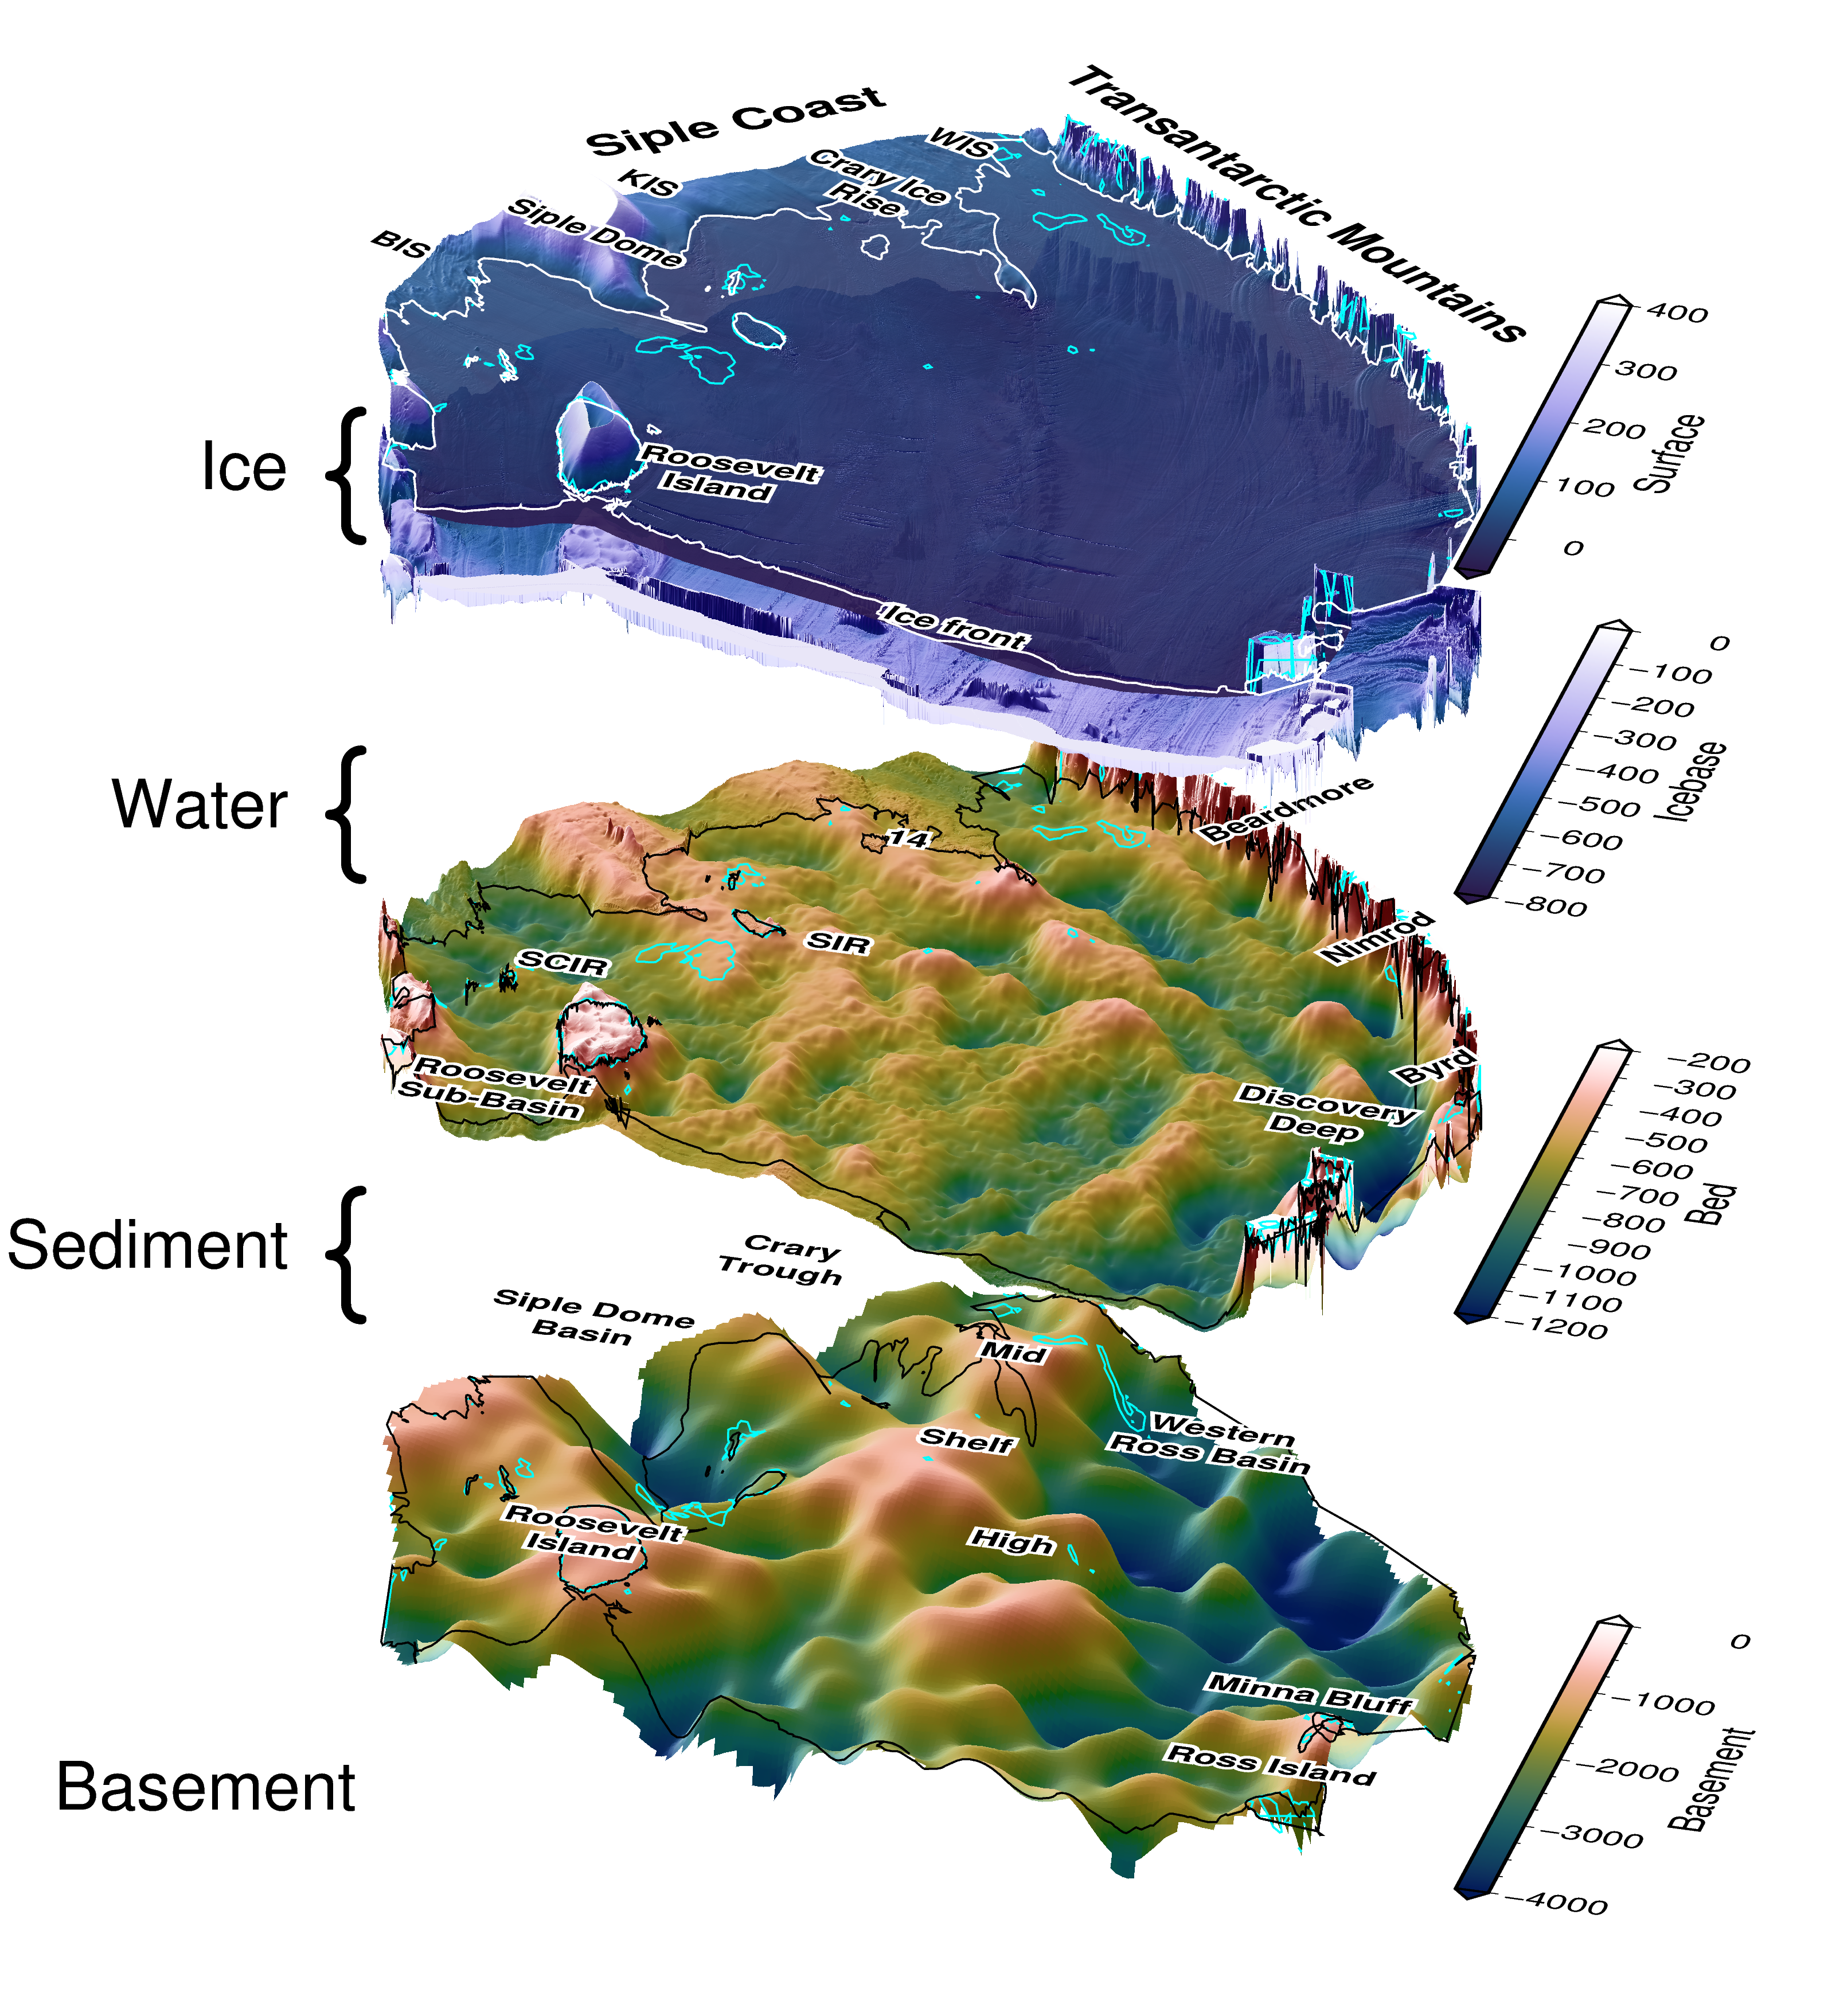
\includegraphics[width=.99\textwidth]{figures/chp5/3D_stack.png}
    \caption[3D perspective view of Ross Ice Shelf]{A 3D perspective view of the structure of the Ross Ice Shelf. Starting at the top, ice surface, and ice base from BedMachine v3 \citep{morlighemdeep2020, morlighemmeasures2022}, inverted bathymetry results from Chapter \ref{ch:4}, and basement topography from Chapter \ref{ch:2}. Grounding line shown in all layers if from \citet{morlighemmeasures2022}. Bright blue contour shows 20~m water column thickness. Note each layer has an independent vertical exaggeration to aid in visualization. Acronyms: BIS: Bindschadler Ice Stream, KIS: Kamb Ice Stream, WIS: Whillans Ice Stream, SCIR: Shirase Coast Ice Rumples, SIR: Steershead Ice Rise.}
    \label{fig:chp5_3D_stack}
\end{figure}


\subsection[Past and future implications]{Constraining past and future ice sheet behaviour\sectionmark{Past and future implications}}
% Past/future pinning points
%     with thicker ice, where was the RIS likely pinned?
%     As ice thins and earth rebounds, where will new pinning points emerge?
% Newly identified basement highs
%     likely subareal during Oligocene ice initialization,
%     would have been major pinning points, similar to Roosevelt Island
%     possibly created ice flow divide between EANT and WANT as seen in Ross Sea sediment record
%     effect on total ice mass calculations for early ice sheet
% Bathymetry features
%     might show depositional / erosional remnants of past retreats/readvances
%     insights into saloon door vs swinging gate mechanism of retreat

While the above geologic controls on the ice sheet likely existed in the past and will continue into the future, our study has implications that are exclusive to past or future ice sheet configurations. The pinning points we discussed, and the regions of thin draft, were all likely pinning points during periods of thicker ice. Since the Last Glacial Maximum ($\sim22$~ka) retreat of the grounding line from the outer shelf edge has been primarily controlled by the physiography of the bed, as well as its geologic composition \citep{halberstadticesheet2016, andersonseismic2019}. While the retreat dynamics have been well studied in the Ross Sea, where the open ocean conditions allow seismic and high-resolution multi-beam sonar surveying \citep{halberstadticesheet2016, andersonseismic2019}, and drill cores provide sedimentary records \citep{mckayantarctic2016}, under the Ross Ice Shelf there has been very little investigation on retreat dynamics, apart from modelling studies \citep{lowrygeologic2020, kingslakeextensive2018}. Here we have provided the physiography of the region, through the sub-Ross Ice Shelf bathymetry model, enabling insight into the retreat dynamics throughout the Holocene. \\
%Understanding the way in which the Ross Ice Shelf and paleo Ross Ice Sheet responded during past periods of warming is vital to predicting its future response to a warming climate. \\

\subsubsection{Retreat dynamics}
While we don't constrain the age of the sea floor sediments, the general physiography of the sea floor can provide some insights. The eastern side of the ice shelf, apart from Roosevelt Island, shows similar physiography to the eastern Ross Sea, with relatively flat bathymetry without major banks or troughs (Figure \ref{fig:chp5_syntheis_figure}e). There, the subdued bathymetry likely resulted in a stepwise style of grounding line retreat throughout the Miocene, with the stabilizing build-up of grounding zone wedges, followed by decoupling and rapid retreat of 10's of kilometres \citep{bartparadox2017, andersonseismic2019}. The bathymetry of the western Ross Ice Shelf, characterized by depth troughs and shallow banks, is similar to that of the western Ross Sea (Figure \ref{fig:chp5_syntheis_figure}e). There, the retreat style, also controlled by the bathymetry, was continuous and complex, as ice streams followed the bathymetry in a continuous retreat back to the outlet valleys in the Transantarctic Mountains \citep{halberstadticesheet2016, andersonseismic2019}. 
% Retreat style and physiography are interdependent; smooth topography leads to wide ice streams, which when retreating in a stepwise fashion, stagnate and deposit significant sediment volume, adding to the smooth nature of the topography. Conversely, steep topography confines flowing ice, leading to narrow ice streams. These are thought to retreat in a continuous fashion, where a lack of stagnation leads to minimal grounding zone deposition. 
In the western Ross Sea, repeated cycles of advance and retreat within these confined bathymetry troughs led to the scouring of sediments from the inner shelf, and an over-deepened, landward sloping inner shelf \citep{andersonseismic2019}. These contrasting styles of retreat proposed for the eastern and western Ross Ice Shelf may be in part responsible for the varied bathymetry found on either side of the ice shelf. The above section discussed our bathymetry results in relation to past and future ice dynamics. Next, we discuss the implication of our basement topography on the glacial history of the region. \\

\subsubsection{Glacial initialization}
During the Oligocene, the Ross Embayment contained a long and broad mountain range emergent above sea level, trending N-S from the Ross Sea through the ice shelf. This feature was first recognized from the drill cores of DSDP (Deep Sea Drilling Project) site 270 in the Ross Sea \citep[Figure \ref{fig:chp5_syntheis_figure}f, ][]{leckielate1983}, where a 400~m sedimentary sequence with depositional environments ranging from above sea level to $\sim500$~m below sea level was found, dating from late Oligocene to early Miocene \citep{kulhanekrevised2019}. Beneath this sequence was crystalline basement. The broad dome-like shape of this basement high was revealed by shipborne seismic surveys \citep{brancolinidescriptive1995}, which imaged a similar basement high further north. These basement features were termed the Northern and Southern Central High. Seismic data also revealed small U-shaped channels within the acoustic basement, which were attributed to alpine glaciation \citep{desantisseismic1995}. Off the flanks of these fault-bound basement highs, wider troughs in the basement were imaged and attributed to the erosion of ice streams flowing off these basement highs. During the late Oligocene, ice caps nucleated on these subaerial basement features \citep{desantisseismic1995, olivettiice2023}. Thermal subsidence following the onset of mid-Cretaceous West Antarctic Rift System extension \citep{karnergravity2005, wilsonwest2009} gradually submerged these basement highs \citep{desantiseastern1999, olivettiice2023}. In addition to the North and South Central High features in the Ross Sea, paleotopographic reconstructions of the Oligocene \citep{paxmanreconstructions2019, wilsonantarctic2012} have predicted the continuation of this broad subaerial mountain range under the Ross Ice Shelf. Our depth to magnetic basement (Chapter \ref{ch:2}) provided the first observations of the feature, which we termed the Mid Shelf High, beneath the Ross Ice Shelf (Figure \ref{fig:chp5_syntheis_figure}f). \\

The strong continuity of the Mid Shelf High with the Ross Sea's Central High suggests that these features have similar histories. We propose the three blocks of the Mid Shelf High were emergent and hosted ice caps in the Oligocene. Following their submersion, likely in the latest Oligocene \citep{olivettiice2023} these features would have acted as major bathymetry pinning points, similar to the modern Roosevelt Island. We suggest this chain of shallow basement blocks formed a long-lasting catchment divide of both sediment transport and ice flow between East and West Antarctica. This divide has been predicted as far back as the Paleogene, from distinct microfossil assemblages on either side of the Ross Embayment \citep{coenenpaleogene2019}. Since the Last Glacial Maximum, the Central High has been thought to be an ice flow divide, separating ice originating from the East and West Antarctic Ice Sheets \citep{liapatite2020, lichtupb2014, lichtprovenance2005}. The prominent Mid Shelf High / Central High appears to have played a central role in the history of the Ross Embayment since the Oligocene. 

% \section{Insights into tectonic and geologic histories}
% direct evidence of West Antarctic Rift System extension
% new evidence of active divergent tectonics within West Antarctica
% additional sediment thickness effects paleotopo reconstructions
% bathymetry trough possible indicator of central TAM uplift style


\section{Future work}
Here we provide several suggestions for future research and fieldwork related to this thesis. A primary piece of future work resulting from this thesis should be the incorporation of the updated bathymetry into a sub-ice shelf circulation model. 
To access the sensitivity of sub-shelf circulations to bathymetry, models should be run for our mean bathymetry model, as well as the upper and lower ranges of our uncertainties, as defined by the mean model plus and minus the spatial uncertainty we present (Figure \ref{fig:chp5_uncertainty_limits}). 
% Ideally, this would incorporate the spatially variable uncertainty of the bathymetry. 
To better improve the bathymetry model and reduce uncertainties, we suggest three alternatives for field seasons on the Ross Ice Shelf. 

\begin{enumerate}
    \item Collect additional seismic depth measurements along the Transantarctic Mountain front. This would serve to lower uncertainties in the bathymetry associated with the nearby steep topography. A traverse-style field season would be best for this to accommodate the linear nature of the grounding zone. Collecting occasional cross lines, running perpendicular to the grounding line, would likely image the range front faults, commonly inferred by only rarely imaged. 
    \item A seismic survey of the central block of the Mid Shelf High (Figure \ref{fig:chp5_syntheis_figure}f). This survey would accomplish several goals. First, it would fill one of the two major gaps in bathymetry measurements in the central ice shelf, reducing the bathymetry uncertainty. Secondly, it would inform on the nature of the Mid Shelf High as a past pinning point and nucleation site of Oligocene ice caps. Lastly, it would act as a site survey for potential sea-floor drilling. The thin sedimentary cover of the Mid Shelf High may provide a good target for future drilling since a temporally wide-ranging sequence may be concentrated into a thin sedimentary package. Additionally, sampling of the crystalline basement, trace element and provenance analysis will give further insights into 1) the proposed East-West Antarctic geologic boundary along the middle of the Ross Embayment \citep{tintoross2019}, 2) the region's Cretaceous extensional history \citep{olivettiice2023}, and 3) the region's Oligocene to Miocene climatic evolution \citep{olivettiice2023}.
    \item Conduct a regional seismic survey across portions of the Siple Coast to better image the sedimentary basins and basin bounding faults, especially where the faults proposed in Chapter \ref{ch:2} may interact with the ice streams.
\end{enumerate}

We make several suggestions for future inversions based on our comprehensive review of past Antarctic bathymetry gravity inversions. To test the inversion method developed here, it would be useful to perform another  inversion for an ice shelf that has been previously inverted. The three best options would be the Getz Ice Shelf, the Thwaites Glacier, and the Pine Island Glacier. The bathymetry beneath each of these ice shelves has been inverted three separate times, allowing the comparison of several different methods. The Getz Ice shelf bathymetry has been inverted in 2D \citep{weigetz2020, cochrandetailed2020}, and with a 3D frequency-based inversion \citep{millanconstraining2020}. The Thwaites cavity has also been inverted in both 2D \citep{tintoprogressive2011} and 3D, with both the "topo-shift method" \citep{jordangeological2020}, and a frequency-based method \citep{millanbathymetry2017}. Lastly, the Pine Island Glacier bathymetry has been inversion twice with Simulated Annealing \citep{mutosubglacial2016, mutosubglacial2013}, and once with a frequency-based inversion \citep{millanbathymetry2017}. To compare to a wider range of methods, the Thwaites glacier would be optimal. To gain insights into the effectiveness of our uncertainty analysis, Pine Island Glacier should be chosen since spatially variable uncertainty estimates exist from the studies which used Simulated Annealing. \\

Of the major Antarctic ice shelves, there are four that stand out as prime candidates for a future inversion if the goal is to increase our sub-ice shelf bathymetric knowledge. These include the Larsen C Ice Shelf, the Ronne Filchner Ice Shelf, the Riiser-Larsen Ice Shelf, and the Shackleton Ice Shelf.

\begin{enumerate}
    \item Larsen C is the largest ice shelf on the Antarctic Peninsula, yet bathymetry knowledge beneath it is still limited. A bathymetry inversion has been conducted \citep{cochraninversion2012}, but comparison with seismic constraints revealed large uncertainties in the model. A recent constraint compilation and new seismic data \citep{brisbourneupdated2020} make this an ideal candidate without needing any field work. Additional gravity data has also been collected over the ice shelf during 2016, 2017, and 2018 Operation Ice Bridge flights \citep{icebridge2020}. 
    \item The Ronne Filchner is the second-largest ice shelf, yet has not been included in a gravity inversion. An extensive array of seismic constraints, similar to the RIGGS survey of the Ross Ice Shelf exists \citep{rosiernew2018, fretwellbedmap22013}, and gravity data from compiled from Russian airborne and ground-based surveys \citep{aleshkovagravity2000, studingercrustal1999} is accessible as part of the continent-wide AntGG gravity compilation \citep{scheinertnew2016}. 
    \item and 4. The Riiser-Larsen and the Shackelton Ice Shelves are the 5th and 7th largest ice shelves, respectively. To our knowledge, there is no bathymetry knowledge beneath the entirety of either shelf. Gravity data exists for both shelves from the AntGG compilation \citep{scheinertnew2016}. Performing inversions for these shelves would require extensive seismic data acquisition to be adequately constrained.
\end{enumerate}

Lastly, we highlight a few alternative use cases and limitations for our gravity inversion algorithm. While this has been developed for a regional-scale sub-ice shelf application, at its core the inversion is a standard geometric (sometimes referred to as structural) inversion. Therefore, this code can be used to invert any topographic surface of a user-defined density contrast based on input gravity anomaly data. It is compatible with domains ranging from small-scale, local areas, to large domains such as ours ($1000~\times~1000$~km). However, domains significantly larger than ours (continental scale) will introduce inaccuracies due to our use of vertical right-rectangular prisms, which makes assumptions of a planar Earth. For these continental to global scale inversions, vertical prisms should be replaced with spherical prisms (tesseroids), as implemented by \citep{uiedafast2017}. With this, our inversion will work for other applications, such as predicting regional Moho depths, the sediment-basement contact, or determining bed depths beneath grounded ice, under subglacial lakes, or in the open ocean. We hope this code is used by others for these various applications.

\section{Concluding remark}
% - improved geologic knowledge for the sub-RIS
% - provide the necessary modelling boundary conditions to lower uncertainties of future sea level rise
% - provided open sources tools to allow other researchers to conduct this research in other locations

The primary aim of this thesis was to use existing airborne geophysical data to better characterize the geology and physiography beneath Antarctica's Ross Ice Shelf. We used and developed several geophysical techniques to accomplish this. We first used variations in Earth's magnetic field measured over the ice shelf to model the spatial distribution and thickness of sediments beneath the ice shelf. We then developed and extensively tested a geophysical inversion, which uses measurements of Earth's gravity field to model the depth to the seafloor. With this, we created an updated model of the bathymetry beneath the ice shelf. \\

From this geophysically informed knowledge of the upper crust of the sub-Ross Ice Shelf, we were able to draw inferences on the complex interactions between the solid Earth, ocean, and ice for the Ross Embayment. We highlighted the Siple Coast as a location with strong geologic control on ice dynamics, through 1) the distribution of sediments, which control the competency of bedrock material beneath grounded ice, and 2) the location of deep sedimentary basins, which likely supply the ice base with lubricating water and localize the geothermal heat delivered to the ice. Our bathymetry model confirms the findings of past models which show a deep trough spanning from the ice front near Ross Island south along the Transantarctic Mountain Front. This trough likely guides High Salinity Shelf Water from the ice front to the deep grounding zone of the Transantarctic Mountain outlet glaciers, where it induces significant basal melting. Our spatial uncertainty results highlight the Transantarctic Mountain Front as the least-certain portion of the sub-ice shelf bathymetry model. Combined with this region's importance for basal melt, we suggest future seismic surveys target the mountain front. This thesis provides the necessary boundary conditions and estimates of their uncertainties for ice and ocean modellers to better characterize the Ross Ice Shelf's response to past, present, and future changes in the climate. 